\documentclass[]{book}
\usepackage{lmodern}
\usepackage{amssymb,amsmath}
\usepackage{ifxetex,ifluatex}
\usepackage{fixltx2e} % provides \textsubscript
\ifnum 0\ifxetex 1\fi\ifluatex 1\fi=0 % if pdftex
  \usepackage[T1]{fontenc}
  \usepackage[utf8]{inputenc}
\else % if luatex or xelatex
  \ifxetex
    \usepackage{mathspec}
  \else
    \usepackage{fontspec}
  \fi
  \defaultfontfeatures{Ligatures=TeX,Scale=MatchLowercase}
\fi
% use upquote if available, for straight quotes in verbatim environments
\IfFileExists{upquote.sty}{\usepackage{upquote}}{}
% use microtype if available
\IfFileExists{microtype.sty}{%
\usepackage{microtype}
\UseMicrotypeSet[protrusion]{basicmath} % disable protrusion for tt fonts
}{}
\usepackage[margin=1in]{geometry}
\usepackage{hyperref}
\hypersetup{unicode=true,
            pdftitle={Tests multivariados de independencia basados en rangos de los vecinos más cercanos},
            pdfauthor={Hernán David Torres, Olga Lisethe Castellanos  Universidad Nacional de Colombia},
            pdfborder={0 0 0},
            breaklinks=true}
\urlstyle{same}  % don't use monospace font for urls
\usepackage{natbib}
\bibliographystyle{apalike}
\usepackage{longtable,booktabs}
\usepackage{graphicx,grffile}
\makeatletter
\def\maxwidth{\ifdim\Gin@nat@width>\linewidth\linewidth\else\Gin@nat@width\fi}
\def\maxheight{\ifdim\Gin@nat@height>\textheight\textheight\else\Gin@nat@height\fi}
\makeatother
% Scale images if necessary, so that they will not overflow the page
% margins by default, and it is still possible to overwrite the defaults
% using explicit options in \includegraphics[width, height, ...]{}
\setkeys{Gin}{width=\maxwidth,height=\maxheight,keepaspectratio}
\IfFileExists{parskip.sty}{%
\usepackage{parskip}
}{% else
\setlength{\parindent}{0pt}
\setlength{\parskip}{6pt plus 2pt minus 1pt}
}
\setlength{\emergencystretch}{3em}  % prevent overfull lines
\providecommand{\tightlist}{%
  \setlength{\itemsep}{0pt}\setlength{\parskip}{0pt}}
\setcounter{secnumdepth}{5}
% Redefines (sub)paragraphs to behave more like sections
\ifx\paragraph\undefined\else
\let\oldparagraph\paragraph
\renewcommand{\paragraph}[1]{\oldparagraph{#1}\mbox{}}
\fi
\ifx\subparagraph\undefined\else
\let\oldsubparagraph\subparagraph
\renewcommand{\subparagraph}[1]{\oldsubparagraph{#1}\mbox{}}
\fi

%%% Use protect on footnotes to avoid problems with footnotes in titles
\let\rmarkdownfootnote\footnote%
\def\footnote{\protect\rmarkdownfootnote}

%%% Change title format to be more compact
\usepackage{titling}

% Create subtitle command for use in maketitle
\newcommand{\subtitle}[1]{
  \posttitle{
    \begin{center}\large#1\end{center}
    }
}

\setlength{\droptitle}{-2em}
  \title{Tests multivariados de independencia basados en rangos de los vecinos
más cercanos}
  \pretitle{\vspace{\droptitle}\centering\huge}
  \posttitle{\par}
  \author{Hernán David Torres, Olga Lisethe Castellanos Universidad Nacional de
Colombia}
  \preauthor{\centering\large\emph}
  \postauthor{\par}
  \predate{\centering\large\emph}
  \postdate{\par}
  \date{martes, 21 de noviembre de 2017}

\usepackage{booktabs}
\usepackage{amsthm}
\usepackage{amssymb}
\usepackage{amsmath}
\usepackage{mathspec}
\providecommand{\abs}[1]{\lvert#1\rvert}
\makeatletter
\def\thm@space@setup{%
  \thm@preskip=8pt plus 2pt minus 4pt
  \thm@postskip=\thm@preskip
}
\makeatother

\begin{document}
\maketitle

{
\setcounter{tocdepth}{1}
\tableofcontents
}
\chapter{INTRODUCCIÓN}\label{introduccion}

\begin{quote}
Se exponen, a continuación, algunos tests multivariados de independencia
entre dos vectores aleatorios de dimensión arbitraria usados,
convenientemente, en situaciones de \emph{\emph{HDLSSD}}.
\citep{sarkar2017some}
\end{quote}

\chapter{¿QUÉ ES HDLSSD?}\label{intro}

Previo a lo anterior, es importante mencionar que \emph{\emph{High
Dimensional Low Sample Size Data}} \emph{\emph{HDLSSD}} refiere, como su
nombre lo indica, a las situaciones en las cuales se tiene alta
dimensionalidad (gran cantidad de variables) y tamaños muestrales
pequeños.

\chapter{EL PROBLEMA}\label{el-problema}

Se han desarrollado muchos tests estadísticos ---tanto paramétricos como
no paramétricos --- para probar la independencia entre 2 vectores
aleatorios, pero dichos test no son aplicables en casos de alta
dimensionalidad y de muestras pequeñas.

\section{Desarrollo teórico}\label{desarrollo-teorico}

En las situaciones tratadas se consideran \emph{\emph{n}} realizaciones
independientes,

\[
 z_{1} =
\begin{pmatrix} x_1\\
y_1\\
\end{pmatrix} 
 ,  z_{2} =
\begin{pmatrix} x_2\\
y_2\\
\end{pmatrix}, ... ,    z_{n} =
\begin{pmatrix} x_n\\
y_n\\
\end{pmatrix},
\]

de un vector aleatorio continuo \[ Z = \mathbf{\begin{pmatrix} X\\
Y\\
\end{pmatrix}},\] donde \(\mathbf{X}\) \(\in\) \(\mathcal{X}\)
\(\subseteq\) \(\mathbb{R}^p\) y \(Y\) \(\in\) \(\mathcal{Y}\)
\(\subseteq\) \(\mathbb{R}^q\)

\section{Tests existentes}\label{tests-existentes}

\begin{longtable}[]{@{}ccl@{}}
\caption{Parangón de los tests propuestos hasta el
momento.}\tabularnewline
\toprule
\begin{minipage}[b]{0.25\columnwidth}\centering\strut
\emph{Test paramétricos}\strut
\end{minipage} & \begin{minipage}[b]{0.10\columnwidth}\centering\strut
\strut
\end{minipage} & \begin{minipage}[b]{0.56\columnwidth}\raggedright\strut
\emph{Test no paramétricos}\strut
\end{minipage}\tabularnewline
\midrule
\endfirsthead
\toprule
\begin{minipage}[b]{0.25\columnwidth}\centering\strut
\emph{Test paramétricos}\strut
\end{minipage} & \begin{minipage}[b]{0.10\columnwidth}\centering\strut
\strut
\end{minipage} & \begin{minipage}[b]{0.56\columnwidth}\raggedright\strut
\emph{Test no paramétricos}\strut
\end{minipage}\tabularnewline
\midrule
\endhead
\begin{minipage}[t]{0.25\columnwidth}\centering\strut
Basado en el estadístico Wilk\strut
\end{minipage} & \begin{minipage}[t]{0.10\columnwidth}\centering\strut
\emph{\emph{Univariados}}\strut
\end{minipage} & \begin{minipage}[t]{0.56\columnwidth}\raggedright\strut
Estadístico de Spearman \(\rho\) y Estadístico de Kendall \(\tau\)\strut
\end{minipage}\tabularnewline
\begin{minipage}[t]{0.25\columnwidth}\centering\strut
Prueba de la raíz más grande de Roy\strut
\end{minipage} & \begin{minipage}[t]{0.10\columnwidth}\centering\strut
\strut
\end{minipage} & \begin{minipage}[t]{0.56\columnwidth}\raggedright\strut
Test basado en cuadrantes estadísticos\strut
\end{minipage}\tabularnewline
\begin{minipage}[t]{0.25\columnwidth}\centering\strut
Traza de Hotelling-Lawley\strut
\end{minipage} & \begin{minipage}[t]{0.10\columnwidth}\centering\strut
\emph{\emph{Multivariados}}\strut
\end{minipage} & \begin{minipage}[t]{0.56\columnwidth}\raggedright\strut
Extensión del test de cuadrantes para mayores dimensiones mediantes
interdirecciones\strut
\end{minipage}\tabularnewline
\begin{minipage}[t]{0.25\columnwidth}\centering\strut
Traza de Pillai-Bartlett\strut
\end{minipage} & \begin{minipage}[t]{0.10\columnwidth}\centering\strut
\strut
\end{minipage} & \begin{minipage}[t]{0.56\columnwidth}\raggedright\strut
Generalizaciones multivariadas de los test basados en Spearman y
Kendall.\strut
\end{minipage}\tabularnewline
\begin{minipage}[t]{0.25\columnwidth}\centering\strut
\strut
\end{minipage} & \begin{minipage}[t]{0.10\columnwidth}\centering\strut
\strut
\end{minipage} & \begin{minipage}[t]{0.56\columnwidth}\raggedright\strut
Generalizaciones del cuadrante estadístico usando signos espaciales y
rangos\strut
\end{minipage}\tabularnewline
\bottomrule
\end{longtable}

\section{Tests aplicables a HDLSS}\label{tests-aplicables-a-hdlss}

Para manipular datos HDLSS en distintas áreas de investigación, se han
desarrollado algunos tests de independencia entre dos vectores, basados
en distancias \emph{inter-point}; sea \(d_{x}\) y \(d_{y}\) medidas de
distancia en \(\mathcal{X}\) y \(\mathcal{Y}\), respectivamente; y, para
toda \((i,j)\), definimos
\[ d_{ij}^x = d_x(x_i, x_j), \\ d_{ij}^y = d_y(y_i, y_j). \]

En la mayoría de los tests presentados, a continuación, se utiliza
distancias euclidianas en \(\mathcal{X}\) y \(\mathcal{Y}\) como
\(d_{x}\) y \(d_{y}\) , respectivamente.

\chapter{TESTS BASADO EN GRAFOS}\label{tests-basado-en-grafos}

\begin{itemize}
\item
  \textbf{\emph{Grafo simple:}} Conjunto de \emph{nodos} unidos por
  enlaces llamados \emph{aristas}.
\item
  \textbf{\emph{Grafo completo}}: Grafo simple donde \emph{cada par de
  vértices} está conectado por una \emph{arista}. Tiene \(n(n-1)/2\)
  aristas. Grafo regular de grado \(n-1\)
\item
  \textbf{\emph{Grafo de arcos ponderados}}: Grafo con asignaciones de
  pesos en cada arco.
\end{itemize}

\begin{figure}

{\centering 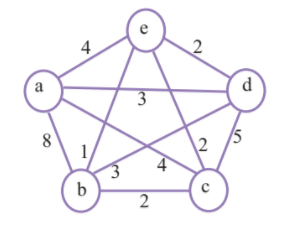
\includegraphics[width=260,height=240]{grafo_completo} 

}

\caption{Grafo completo ponderado}\label{fig:unnamed-chunk-1}
\end{figure}

\section{Conceptos en teoría de
grafos}\label{conceptos-en-teoria-de-grafos}

\begin{itemize}
\tightlist
\item
  \textbf{\emph{Subgrafo:}} Cuyo conjunto de vértices(como el de
  aristas) es un subconjunto del de grafo original.
\item
  \textbf{\emph{Camino:}} Secuencia de vértices dentro de un grafo tal
  que exista una arista entre cada vértice y el siguiente.
\item
  \textbf{\emph{Árbol:}} Donde cualesquiera dos vértices están
  conectados por exactamente \emph{un camino}.
\end{itemize}

\begin{figure}

{\centering 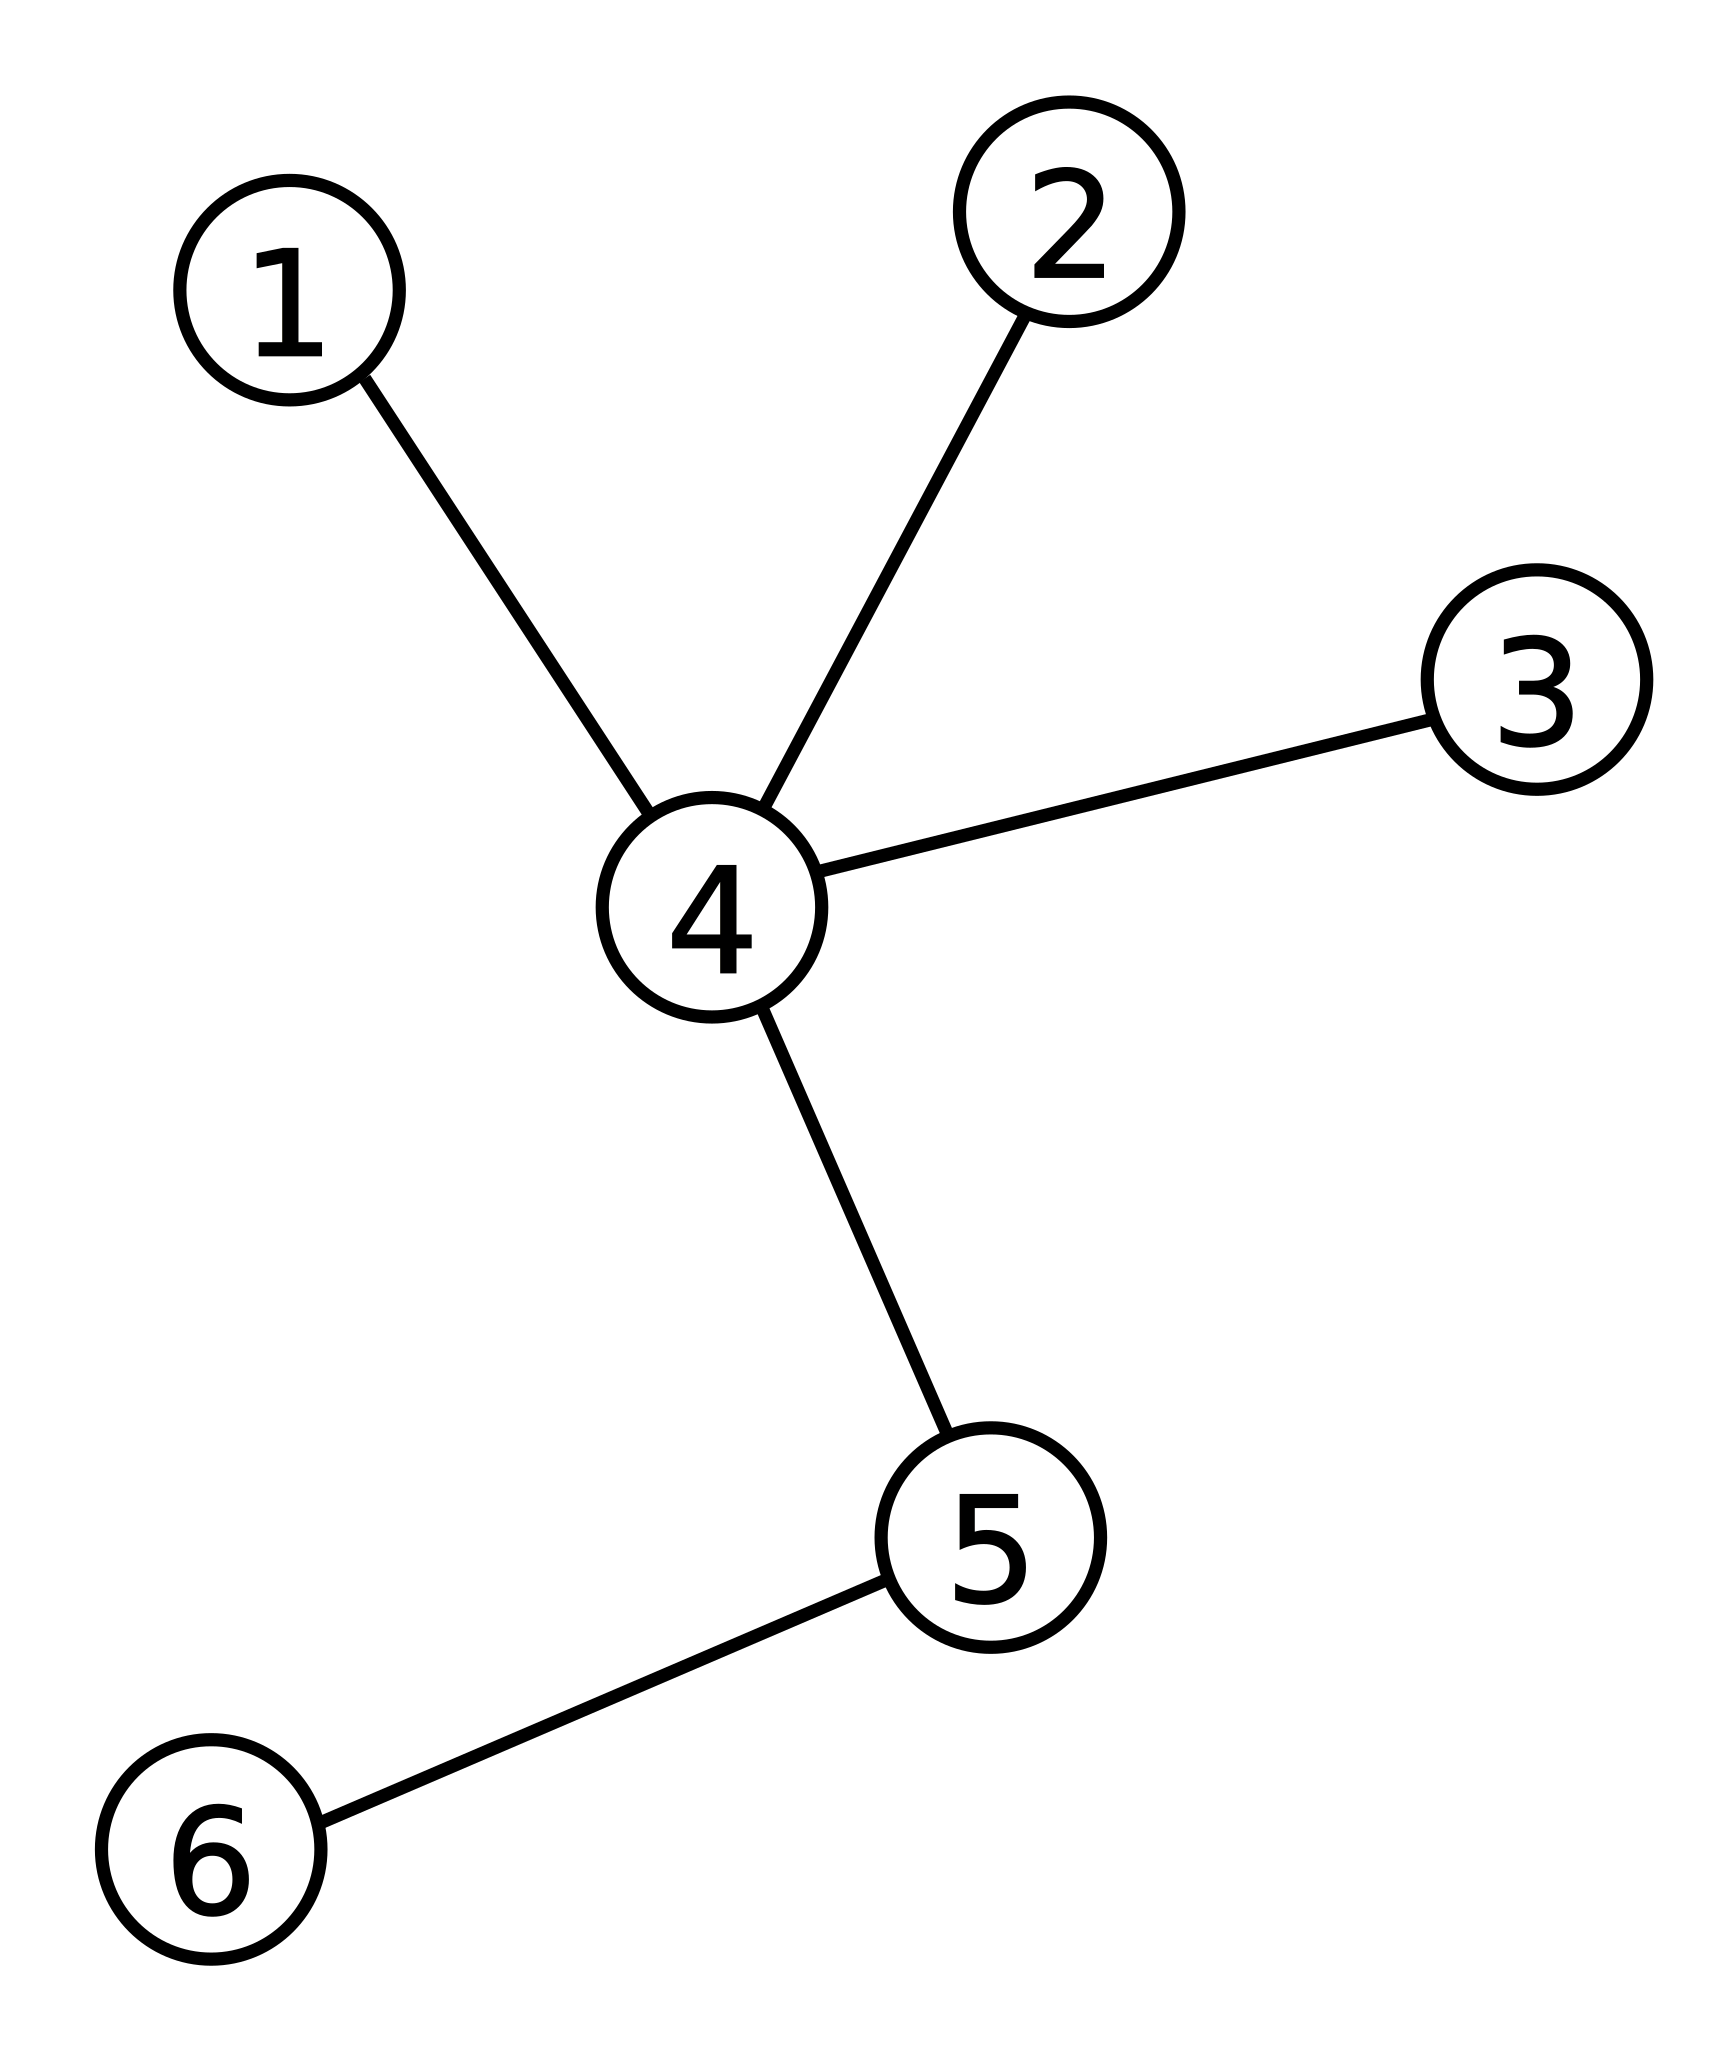
\includegraphics[width=260,height=240]{Tree_graph} 

}

\caption{Árbol}\label{fig:unnamed-chunk-2}
\end{figure}

\section{Precisiones del test}\label{precisiones-del-test}

Se consideran dos grafos completos de arcos ponderados
\(\mathcal{G}_{\mathbf{x}}\) y \(\mathcal{G}_{\mathbf{y}}\) con nodos
\(\mathbf{x_1,...,x_n}\) y \(\mathbf{y_1,..., y_n}\), respectivamente,
donde \(d_{i,j}^{\mathbf{x}}\) (y, correspondientemente,
\(d_{i,j}^{\mathbf{y}}\)) es la ponderación asociada con el lado que
conecta a \(\mathbf{x}_i\) y \(\mathbf{x}_j\) (y, paralelamente, con
\(\mathbf{y}_i\) y \(\mathbf{y}_j\)) \citep{friedman1983graph}

\section{Grafo K vecinos más
próximos}\label{grafo-k-vecinos-mas-proximos}

El gráfico K-NN en \(\mathcal{G}_{\mathbf{x}}\) tiene un arco entre
\(x_i\) y \(x_j\), si \(x_i\) es uno de los primeros K vecinos de
\(x_j\) o viceversa; y, análogamente, para \(\mathcal{G}_{\mathbf{x}}\).

\begin{figure}

{\centering 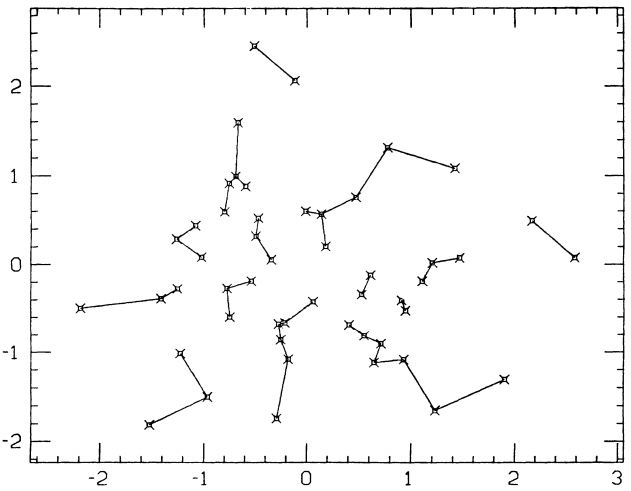
\includegraphics[width=450,height=320]{1-nn} 

}

\caption{1-NN 50 obs. Normal bivariada}\label{fig:unnamed-chunk-3}
\end{figure}

\section{Grafo 5-NN}\label{grafo-5-nn}

\begin{figure}

{\centering 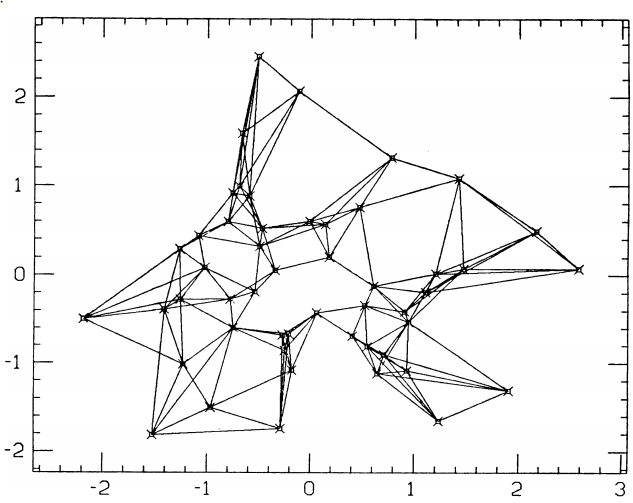
\includegraphics[width=450,height=320]{5-nn} 

}

\caption{5-NN en 50 obs. Normal bivariada}\label{fig:unnamed-chunk-4}
\end{figure}

\section{El árbol recubridor mínimo
(MST)}\label{el-arbol-recubridor-minimo-mst}

Es un subgrafo que tiene que ser un árbol y contener todos los vértices
del grafo inicial y, a la vez, será el de la menor suma de los pesos.

\begin{figure}

{\centering 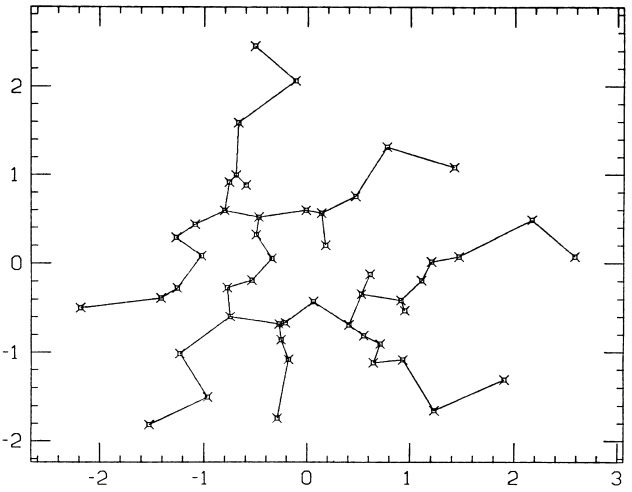
\includegraphics[width=450,height=320]{1-MST} 

}

\caption{1-MST en 50 obs. Normal bivariada}\label{fig:unnamed-chunk-5}
\end{figure}

\section{Grafo 5-MST}\label{grafo-5-mst}

El r-MST, \(r={1, 2,...,K}\), es un árbol recubridor mínimo que no
comparte arco alguno con ninguno de los r-1 anteriores.

\begin{figure}

{\centering 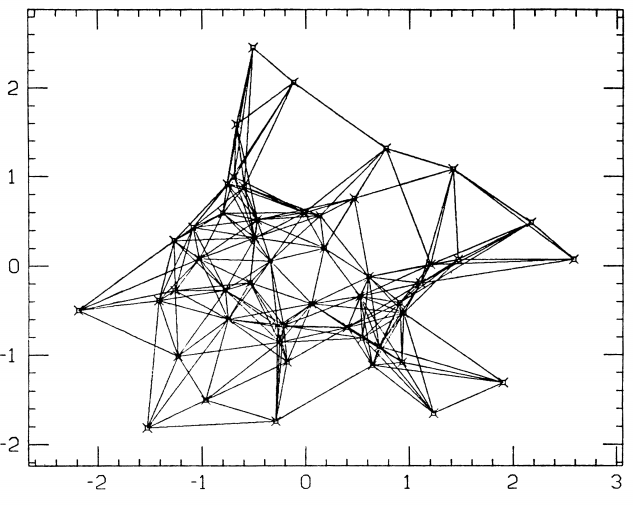
\includegraphics[width=450,height=320]{5-MST} 

}

\caption{5-MST en 50 obs. Normal bivariada}\label{fig:unnamed-chunk-6}
\end{figure}

\section{Test estadístico}\label{test-estadistico}

Sea \(\tau_x^k\) y \(\tau_y^k\) el K-MST o el K-NN sobre el grafo
completo \(\mathcal{G}_{\mathbf{x}}\) y \(\mathcal{G}_{\mathbf{x}}\),
respectivamente.

Se define lo siguiente para determinar el número de arcos en común.

\[a_{ij}=  \left\{
  \begin{array}{ll}
 1 &  \mathcal{Sí} \ (i,j)\in \mathcal{G}_{\mathbf{x}}  \\
 0 &  \mathcal{e.o.c.} \\ 
 \end{array}
\right.
\] De la misma forma se definen los \(b_{i,j}\) basados en las
distancias de \(\mathcal{Y}\).

El estadístico correspondiente es:

\[T_{RF} = \displaystyle \sum_{i=1}^n \sum_{j=1}^n a_{ij}b_{ij}\]

\section{Test estadístico libre de distribución basado en
grafos}\label{test-estadistico-libre-de-distribucion-basado-en-grafos}

Pequeñas distancias en \(\mathcal{x}\) corresponden a pequeñas
distancias en \(\mathcal{y}\)

Seleccionamos un recorrido aleatorio del árbol, donde en cada paso
comenzamos en un nodo ya visitado,\(i \in V= {1,2,...,n}\), y avanzamos
hacia un nuevo nodo,\(j \in V^c\),. Por lo tanto, el árbol se recorre en
\(n-1\) pasos. Se calcula el rango R\_i en cada \(d_{i,j}^{\mathbf{y}}\)
y se obtienen \(n-2\) rangos.

Y se usa el siguiente estadístico

\[T_{RT} =  -2 \displaystyle \sum_{i=1}^{n-2} log(\dfrac{R_j}{n-i})\]

\section{Ejemplo}\label{ejemplo}

\begin{figure}

{\centering 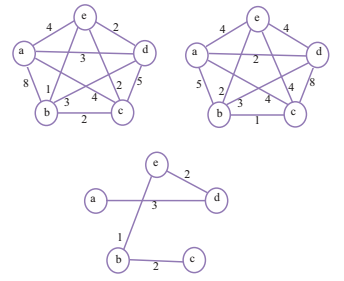
\includegraphics[width=500,height=450]{test6} 

}

\caption{Ejemplo de juguete}\label{fig:unnamed-chunk-7}
\end{figure}

\section{Algoritmo de Prim}\label{algoritmo-de-prim}

Permite encontrar un árbol recubridor mínimo de un grafo no dirigido y
completo. 1. Se selecciona el arco con menor peso. 2. Aumentar el árbol
por un lado: De las posibles uniones que pueden conectar el árbol a los
vértices que no están aún en el árbol, encontrar el lado de menor
distancia y unirlo al árbol. 3. Repetir el paso 2 (hasta que todos los
vértices pertenezcan al árbol) \citep{heller2012consistent}

\section{Test modificado libre de
distribución}\label{test-modificado-libre-de-distribucion}

A causa de la selección aleatoria del recorrido, el anterior test puede
determinar inferencias engañosas. Para eso se usa un recorrido
sistemático siguiendo el algoritmo de Prim. \citep{heller2012consistent}

Y se usa el estadístico T\_\{RT\} de la misma notación; en vez de
\(R_i\), se usa \(R_o\) para distiguir la selección sitematizada de la
aleatoria.

\[T^{o} = -2 \displaystyle \sum_{i=1}^{n-2} log \left( \dfrac{R_i^o}{n-i}\right)\]

Sin embargo, los anteriores tests se desempeñan deficientemente en caso
de estar \(d_{i,j}^{\mathbf{y}}\) y \(d_{i,j}^{\mathbf{y}}\)
negativamente relacionada. El problema es afrontado haciendo

\[R_i^{r} = n-i+1- R_o^i\] para \(i= 1, 2, ... , n-2\)

Así

\[ T^{r} = -2 \displaystyle \sum_{i=1}^{n-2} log \left( \dfrac{R_i ^r}{n-i}\right)\]

\chapter{TEST BASADO EN CORRELACIÓN DE
DISTANCIA}\label{test-basado-en-correlacion-de-distancia}

Para todas las distribuciones con primeros momentos finitos, la
correlación de distancias \(\mathcal{R}\) generaliza la idea de
correlación de dos maneras fundamentales \citep{szekely2007measuring}:

\begin{itemize}
\tightlist
\item
  \(\mathcal{R} \mathbf{(X, Y)}\) se define para \(\mathbf{X}\) y
  \(\mathbf{Y}\) en dimensiones arbitrarias;
\item
  \(\mathcal{R} \mathbf{(X, Y)}\) = 0 caracteriza la independencia de
  \(\mathbf{X}\) y \(\mathbf{Y}\)
\end{itemize}

Para probar \(H_0: f_{x,y}= f_xf_y\) vs. \(H_A: f_{x,y}\neq f_xf_y\)

\section{Precisiones del test}\label{precisiones-del-test-1}

Para cada par \((i,j)\) con \((i \leq i \neq j \leq n)\) se define:

\[A_{i,j} = d_{i,j}^x - d_{i,0}^x - d_{0,j}^x + d_{0,0}^x\]

Con:

\[d_{i,0}^x =  n^{-1} \sum_{j=1}^n d_{i,j}^x\]

\[d_{0,j}^x = n^{-1} \sum_{i=1}^n d_{i,j}^x\]

\[d_{0,0}^x = n^{-1} \sum_{i=1}^n d_{i,0}^x =  n^{-1} \displaystyle\sum_{j=1}^n d_{0,j}^x \]

De la misma forma se definen los \(B_{i,j}\) basados en las distancias
de \(Y\).

\section{Estadístico}\label{estadistico}

El estadístico se define como:

\[T_{dCov}=\dfrac{ \displaystyle \left[ \sum_{i=1}^n \sum_{j=1}^n A_{i,j}B_{i,j} \right]}{ \displaystyle  \left[  \sum_{i=1}^n \sum_{j=1}^n  A_{i,j}^2  \sum_{i=1}^n \sum_{j=1}^n B_{i,j}^2 \right]^{1/2}}  \]

Y es consistente para muestras grandes, pero no es eficaz cuando
\(d_{i,j}^\mathbf{x}\) y \(d_{i,j}^\mathbf{y}\) son correlacionadas
negativamente.

\chapter{\texorpdfstring{TEST BASADO EN DISTANCIAS \(L_1\) Y KULLBACK-
LEIBLER}{TEST BASADO EN DISTANCIAS L\_1 Y KULLBACK- LEIBLER}}\label{test-basado-en-distancias-l_1-y-kullback--leibler}

Se consideran dos enfoques definidos cuando la distribución empírica de
las variables es restringida a particiones finitas. Estos tests resultan
ser fuertemente consistentes.

\section{\texorpdfstring{Estadístico basado en
\(L_1\)}{Estadístico basado en L\_1}}\label{estadistico-basado-en-l_1}

Se denota \(v_n^{\mathbf{Z}}\) la distribución de \((x,y)\);
\(\mu_n^{\mathbf{X}}\) y \(\mu_n^{\mathbf{Y}}\) distribuciones de \(x\)
y \(y\).

Sean \(P_n ={A_{n,1}, ... , A_{n,m_n}}\) y
\(Q_n ={B_{n,1}, ... , B_{n,m'_n}}\) particiones disyuntas de \(X\) y
\(Y\).

Toda vez que \(A\) y \(B\) son subconjuntos de Borel, tenemos
\[\nu_n(A \times B) = n^-1 \# \{i: (X_i, Y_i) \in A \times B, i = 1,...,n\}\]
\[\mu_n^{\mathbf{X}}(A) = n^-1 \# \{i: X_i \in A , i = 1,...,n\}\]
\[\mu_n^{\mathbf{Y}}(B) = n^-1 \# \{i: Y_i \in  B, i = 1,...,n\}\]

Se define el estadístico \(L_1\) como

\[\displaystyle \sum _{A\in P_n} \sum_{B \in Q_n} |\mu_n^{\mathbf{X}} (A \times B) - \mu_n^{\mathbf{X}}(A)\mu_n^{\mathbf{Y}}(B)|\]

y el estadístico \textbf{Kullback- Leibler o log-verosimilitud}

\[ \displaystyle \sum_{A\in P_n} \sum_{B\in Q_n} \mu_n^z(A \times B) log \left[ \dfrac{\mu_n^z(A \times B)}{{\mu_n^x(A) \mu_n^y(B)}}\right]\]

Rechaza \(H_0 : v= \mu_n^x \times \mu_n^Y\) para valores grandes del
estadístico.

\chapter{TEST BASADO EN KERNEL
REPRODUCTOR}\label{test-basado-en-kernel-reproductor}

\textbf{Espacio de Hilbert con núcleo (Kernel) reproductor:} Es un
espacio de Hilbert de funciones para las cuales todas las aplicaciones
son operadores lineales.

\section{Precisiones del test}\label{precisiones-del-test-2}

Se propone un test basado en el hecho de que \(\mathbf{X}\) y
\(\mathbf{Y}\) son independientes si y solo si \(f(\mathbf{X})\) y
\(g(\mathbf{Y})\) son incorrelacionadas para todo \(f\)
\in \mathcal{H_X} \$ y \(g\) \in \mathcal{H_Y}\$ donde \$
\mathcal{H_X}\$ y \(\mathcal{H_Y}\) son espacios del núcleo reproductor

El estadístico está definido como:

\[T_{GG}= n^{-2} \left( \displaystyle \sum_{i=1}^n \sum_{j=1}^n  \alpha_{i,j} \beta_{i,j} \right) - 2n^{-3} \displaystyle \sum_{i=1}^n \left(  \sum_{j=1}^n \alpha_{i,j}  \right) \left(  \sum_{j=1}^n \beta_{i,j}  \right) +  n^{-4}\left(      
 \displaystyle   \sum_{i=1}^n \sum_{j=1}^n \alpha_{i,j} \right)  \left(     \sum_{i=1}^n  \sum_{j=1} ^n \beta_{i,j}  \right) \]

Con

\[\alpha_{i,j} = k^{ \mathcal{\mathbf{x}}} (\mathcal{\mathbf{x}}_i, \mathcal{\mathbf{x}}_j)\]

\[\beta_{i,j} = k^{ \mathcal{\mathbf{y}}} (\mathcal{\mathbf{y}}_i, \mathcal{\mathbf{y}}_j)\]

Para \(k^{ \mathcal{\mathbf{x}}}\) y \(k^{ \mathcal{\mathbf{y}}}\) las
núcleos reproductores asociados a \(\mathcal{H_X}\) y \(\mathcal{H_Y}\)

\chapter{TEST BASADO EN ASOCIACIÓN DE RANGOS
DISTANCIAS}\label{test-basado-en-asociacion-de-rangos-distancias}

Se propone un test basado en el estadístico \(\chi^2\) de Pearson
calculado en una tabla de contingencia basada en distancia por pares,
donde se asigna cada \(\mathbf{z_k}\) (\(k \neq i, j\)) a una celda
según coresponda.

\begin{figure}
  
  {\centering 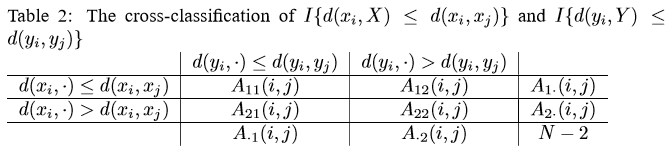
\includegraphics[width=450,height=220]{test5} 
  
  }
  
  \caption{Tabla de contingencia para la clasificación cruzada}\label{fig:unnamed-chunk-8}
  \end{figure}

Y así se define el test estadístico:

\[ T_{HHG} = \displaystyle  \sum_{i=1}^n  \sum_{j (\neq i) =1}^n S_{ij} \]

\chapter{TEST PROPUESTO POR EL AUTOR}\label{test-propuesto-por-el-autor}

\begin{itemize}
\item
  Para cada \(z_i = \binom {x_i}{y_i}\) se organizan los otros \(z_js\)
  \((j\neq i)\) según sus x- distancias de \(Z_i\). para
  \(k= 1,2, ... , n-1\).
\item
  Sea \(z_{ik}\) el k-ésimo vecino más cercano de \(z_i\) \$ (d\_\{i,
  i\_1\}\^{}x \leq d\_\{i, i\_2\}\^{}x \leq \ldots{} \leq d\_\{i,
  i\_\{n-1\}\}\^{}x )\$ .
\item
  Sea \(R_{i,1}\) el rango de \(d_{i,i_1}^y\)\\
  la y-distancia correspondiente a vecino mas cercano x de \(z_i\) en el
  conjunto de
  \[ (d_{i, i_1}^y  ,  d_{i, i_2}^y ,...  , d_{i, i_{n-1}}^y  )\]
\item
  Para \(k= 2, ..., n-2\), \(R_{i,k}\) es definido como el rango de
  \(d_{i,i_k}^y\) , la y-distancia correspondiente al k-ésimo x-vecino
  más cercano de \(Z_i\), en el conjunto
  \({d_{i,i_k}^y, ... , d_{i, i_{n-1}}^y}\) que contiene \(n-k\) de las
  y-distancias.
\item
  Se repite el procedimiento para todos los valores de
  \(i = 1, 2,..., n\)
\end{itemize}

\section{Rangos retrospectivos}\label{rangos-retrospectivos}

\begin{itemize}
\item
  Se define rangos retrospectivos como: \(R_{i,k}^r = n-k+1 - R_{i,k}\)
  para \(i=1,2,...,n\) y \(k = 1,2, ... , n-2\).
\item
  Para alguna función monótona adeduada \(\varphi\) en \([0,1]\),
\end{itemize}

\$T\_1=-2\displaystyle \sum\emph{\{i=1 \^{}n\} \sum}\{k=1\}\^{}\{n-2\}
\varphi \left( \dfrac{R_{i,k}}{n-k}\right), \$ y
\(T_2= -2 \displaystyle \sum_{i=1}^n \sum_{k=1}^{n-2} \left( \dfrac{R_{i,k} ^r}{n-k} \right)\)

Miden asociaciones positivas y negativas.

\begin{itemize}
\item
  Se usa \(\varphi(t) = log(t)\)
\item
  Finalmente, \$T= max(T\_1 ,T\_2) \$ es el estadístico usado.
\end{itemize}

\(H_0\) se rechaza para valores grandes de T.

\section{Permutaciones}\label{permutaciones}

Para algún \(i\) fijo, los \(R_{i,j}\)'s son independientes bajo
\(H_0\). \(R_{i,k}\) sigue una distribución uniforme

Para \(i\neq j\) la distribución conjunta de \(R_{i,k}\) y \(R_{j,k}\)
con \(k, k=1,2, ... , n-2\) puede depender de la distribución subyacente
de \(Z\).

Considerando una permutación aleatoria \(\phi\) de
\(\{ 1, 2, ... , n \}\) y usando :

\(Z_1 ^ * = \binom {x_1}{ y_{\phi (1)}}\)

\(Z_2 ^* = \binom {x_2}{ y_{\phi (2)}}\)

. . . \(Z_n ^* = \binom {x_n}{ y_{\phi (n)}}\)

El estadístico es calculado usando estas mismas observaciones

\section{Corregir asimetría del test}\label{corregir-asimetria-del-test}

\(T_{x,y}\) : Rangos de y-distancias de los x-vecinos más cercanos

\(T_{y,x}\) : Rangos de x-distancias de los y-vecinos más cercanos

\[T_sum = T_{x,y} + T_{y,x}\] \[T_{max} = max (T_{x,y}, T_{y,x})\]

\chapter{EJEMPLO CON DATOS REALES}\label{ejemplo-con-datos-reales}

\begin{figure}
  
  {\centering 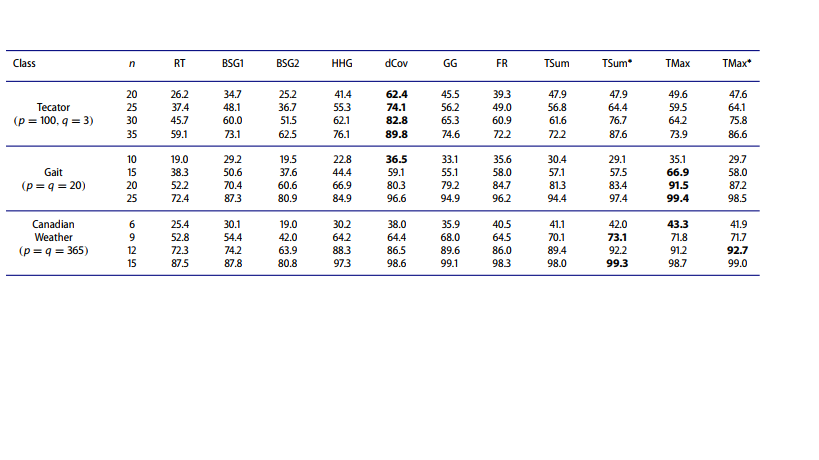
\includegraphics[width=800,height=450]{invento} 
  
  }
  
  \caption{Tabla de contingencia para la clasificación cruzada}\label{fig:unnamed-chunk-9}
  \end{figure}

\chapter{CONCLUSIONES}\label{conclusiones}

\begin{itemize}
\item
  Si bien los test estadísticos presentados son convenientes en el caso
  en el que el número de variables supera el de individuos, aún
  presentan ciertas limitaciones; lo cual motivó al autor al desarrollo
  y presentación de un nuevo método, el cual busca proveer una mejor
  herramienta para probar independencia entre las variables.
\item
  En la construcción del test, se requiere algún tipo de asociación
  entre las x-distancias y las y-distancias, sin embargo, estas
  relaciones se pueden reflejar sólo en sus vecinos más cercanos;
  teniendo en cuenta esto, se propone un test multiescala.
\item
  Si bien, para la implementación de los distintos test se utilizó la
  distancia Euclidiana, es posible emplear otro concepto de distancia.
\end{itemize}

\bibliography{book.bib,packages.bib,referencias.bib}


\end{document}
